\documentclass[]{article}
\usepackage[T1]{fontenc}
\usepackage{lmodern}
\usepackage{amssymb,amsmath}
\usepackage{ifxetex,ifluatex}
\usepackage{fixltx2e} % provides \textsubscript
% use upquote if available, for straight quotes in verbatim environments
\IfFileExists{upquote.sty}{\usepackage{upquote}}{}
\ifnum 0\ifxetex 1\fi\ifluatex 1\fi=0 % if pdftex
  \usepackage[utf8]{inputenc}
\else % if luatex or xelatex
  \ifxetex
    \usepackage{mathspec}
    \usepackage{xltxtra,xunicode}
  \else
    \usepackage{fontspec}
  \fi
  \defaultfontfeatures{Mapping=tex-text,Scale=MatchLowercase}
  \newcommand{\euro}{€}
\fi
% use microtype if available
\IfFileExists{microtype.sty}{\usepackage{microtype}}{}
\usepackage{longtable,booktabs}
\usepackage{graphicx}
% Redefine \includegraphics so that, unless explicit options are
% given, the image width will not exceed the width of the page.
% Images get their normal width if they fit onto the page, but
% are scaled down if they would overflow the margins.
\makeatletter
\def\ScaleIfNeeded{%
  \ifdim\Gin@nat@width>\linewidth
    \linewidth
  \else
    \Gin@nat@width
  \fi
}
\makeatother
\let\Oldincludegraphics\includegraphics
{%
 \catcode`\@=11\relax%
 \gdef\includegraphics{\@ifnextchar[{\Oldincludegraphics}{\Oldincludegraphics[width=\ScaleIfNeeded]}}%
}%
\ifxetex
  \usepackage[setpagesize=false, % page size defined by xetex
              unicode=false, % unicode breaks when used with xetex
              xetex]{hyperref}
\else
  \usepackage[unicode=true]{hyperref}
\fi
\hypersetup{breaklinks=true,
            bookmarks=true,
            pdfauthor={},
            pdftitle={},
            colorlinks=true,
            citecolor=blue,
            urlcolor=blue,
            linkcolor=magenta,
            pdfborder={0 0 0}}
\urlstyle{same}  % don't use monospace font for urls
\setlength{\parindent}{0pt}
\setlength{\parskip}{6pt plus 2pt minus 1pt}
\setlength{\emergencystretch}{3em}  % prevent overfull lines
\setcounter{secnumdepth}{0}
\usepackage{fancyhdr}
\pagestyle{fancy}
\lhead{C-Lyrics - A Word Cloud for Lyrics}
\rhead{\thepage}
\cfoot{Team 6}
\renewcommand{\headrulewidth}{0.4pt}
\renewcommand{\footrulewidth}{0.4pt}

\title{Clyrics - A Word Cloud for Lyrics}
\author{Justine Cocchi\\jcocchi@usc.edu \and Kelsey Fargas\\kfargas@usc.edu \and Mark Krant \\ mkrant@usc.edu\and Milad Gueramian\\gueramia@usc.edu \and Jeff Kang\\kangjr@usc.edu \and Séb Arnold\\arnolds@usc.edu}
\date{30 March 2015}

\title{%
	C-lyrics - A Word Cloud for Lyrics \\
	\large Implementation Design Document}

\begin{document}

\clearpage\maketitle
\thispagestyle{empty}

\pagebreak

\tableofcontents
\setcounter{tocdepth}{3}
\thispagestyle{empty}

\pagebreak

\section{Executive Summary}\label{executive-summary}

C-lyrics is a public website that will generate a word cloud for any
given artist based on the most frequently used words that appear across
all of the artist's published songs. This product will interface with
the EchoNest API which will serve as the database from which we find and
analyze the songs. By clicking on a specific word in the word cloud the
user can see a list of all of the songs that word appears in and how
frequently it occurs in each song. Furthermore, the user can click on
any listed song title to see the complete lyrics for that song with the
original word that was selected from the word cloud highlighted every
time it appears.

C-lyrics is intended for use by the general public. There will be no
login required and there is no stored history of previous searches.
Because of this we will have very low memory requirements and can run
the product off of one server. The user can access C-lyrics using any
device running any OS, assuming it has an internet connection. After
typing in the artist name and selecting the submit button, the word
cloud will be generated and will be able to be shared via Facebook.

\pagebreak

\section{1 Introduction}\label{introduction}

\subsection{\textbf{1.1 Overview}}\label{overview}

The objective of this document is to deliver, demonstrate and document
the first implementation of the C-lyrics software product to the
customer. It includes detailed description of the code base management
policies, mapping to the project management plan, and mappings to the
design document for verification purposes. A startup guide to the
deliverable software is also included to guide the customer

\subsection{\textbf{1.2. Scope}}\label{scope}

The intended audience of this document however is for the client and the
future maintainers of the code base who will presumably be hired by the
client. Ideally, the document should clarify the implementation
techniques by making them predictable given that they follow the prior
documents on design and management and this is the guiding principle
with which the document is drafted. Consequently, some sections will
include designs and descriptions taken from these prior documents on
design and management.

\section{1.3 Definitions and
Acronyms}\label{definitions-and-acronyms}

\begin{longtable}[c]{@{}ll@{}}
\toprule\addlinespace
\begin{minipage}[t]{0.47\columnwidth}\raggedright
Term
\end{minipage} & \begin{minipage}[t]{0.47\columnwidth}\raggedright
Definition
\end{minipage}
\\
\hline
\\\addlinespace
\begin{minipage}[t]{0.47\columnwidth}\raggedright
AJAX
\end{minipage} & \begin{minipage}[t]{0.47\columnwidth}\raggedright
Asynchronous JavaScript And XML. Technology allowing the transfer of
data from between the front- and back-end without reloading the web
page.
\end{minipage}
\\\addlinespace
\begin{minipage}[t]{0.47\columnwidth}\raggedright
API (EchoNest)
\end{minipage} & \begin{minipage}[t]{0.47\columnwidth}\raggedright
API will refer to the EchoNest API. EchoNest is a free API that allows
developers to retrieve lyrics and artist information in web pages and
other programs.
\end{minipage}
\\\addlinespace
\begin{minipage}[t]{0.47\columnwidth}\raggedright
Autocomplete
\end{minipage} & \begin{minipage}[t]{0.47\columnwidth}\raggedright
Autocomplete refers to the functionality addition to the Search Bar,
allowing users to enter minimal characters and choose artists that are
most similar to the string and display a picture of those artists next
to their name.
\end{minipage}
\\\addlinespace
\begin{minipage}[t]{0.47\columnwidth}\raggedright
Autocomplete Delay
\end{minipage} & \begin{minipage}[t]{0.47\columnwidth}\raggedright
A feature designed for the search bar when a user is typing. The delay
refers to the suspending action while the user is typing, making the
request to the server for autocomplete.
\end{minipage}
\\\addlinespace
\begin{minipage}[t]{0.47\columnwidth}\raggedright
Backend
\end{minipage} & \begin{minipage}[t]{0.47\columnwidth}\raggedright
References the PHP backend page
\end{minipage}
\\\addlinespace
\begin{minipage}[t]{0.47\columnwidth}\raggedright
Back to home button
\end{minipage} & \begin{minipage}[t]{0.47\columnwidth}\raggedright
A button redirecting the user to the homepage.
\end{minipage}
\\\addlinespace
\begin{minipage}[t]{0.47\columnwidth}\raggedright
Back to songs button
\end{minipage} & \begin{minipage}[t]{0.47\columnwidth}\raggedright
A button redirecting the user to the songs list page.
\end{minipage}
\\\addlinespace
\begin{minipage}[t]{0.47\columnwidth}\raggedright
Commonly Used Web Browser
\end{minipage} & \begin{minipage}[t]{0.47\columnwidth}\raggedright
Browsers such as Firefox, Safari, Chrome, Explorer, and Quora which come
on mobile phones, tablets and personal computers.
\end{minipage}
\\\addlinespace
\begin{minipage}[t]{0.47\columnwidth}\raggedright
Customer/Client
\end{minipage} & \begin{minipage}[t]{0.47\columnwidth}\raggedright
Dr. William G. Halfond and Sonal Mahajan
\end{minipage}
\\\addlinespace
\begin{minipage}[t]{0.47\columnwidth}\raggedright
GitHub
\end{minipage} & \begin{minipage}[t]{0.47\columnwidth}\raggedright
A web service that provides software version control tools.
www.github.com
\end{minipage}
\\\addlinespace
\begin{minipage}[t]{0.47\columnwidth}\raggedright
Stakeholders
\end{minipage} & \begin{minipage}[t]{0.47\columnwidth}\raggedright
The client and the development team
\end{minipage}
\\\addlinespace
\begin{minipage}[t]{0.47\columnwidth}\raggedright
LOC
\end{minipage} & \begin{minipage}[t]{0.47\columnwidth}\raggedright
acronym: for Lines of Code
\end{minipage}
\\\addlinespace
\begin{minipage}[t]{0.47\columnwidth}\raggedright
KSLOC
\end{minipage} & \begin{minipage}[t]{0.47\columnwidth}\raggedright
a metric that stands for: 1,000(K) Source Lines of Code
\end{minipage}
\\\addlinespace
\begin{minipage}[t]{0.47\columnwidth}\raggedright
Desktop Platform
\end{minipage} & \begin{minipage}[t]{0.47\columnwidth}\raggedright
A screen whose width exceeds 560px
\end{minipage}
\\\addlinespace
\begin{minipage}[t]{0.47\columnwidth}\raggedright
Development Team
\end{minipage} & \begin{minipage}[t]{0.47\columnwidth}\raggedright
All of the individuals whose names appear on the cover of this document.
These persons have collectively put this document together and will
collectively implement the software product described in subsequent
sections.
\end{minipage}
\\\addlinespace
\begin{minipage}[t]{0.47\columnwidth}\raggedright
Facebook
\end{minipage} & \begin{minipage}[t]{0.47\columnwidth}\raggedright
Online social network service where the generated word cloud image may
be shared amongst users.
\end{minipage}
\\\addlinespace
\begin{minipage}[t]{0.47\columnwidth}\raggedright
FR
\end{minipage} & \begin{minipage}[t]{0.47\columnwidth}\raggedright
Functional Requirement
\end{minipage}
\\\addlinespace
\begin{minipage}[t]{0.47\columnwidth}\raggedright
Google Doc
\end{minipage} & \begin{minipage}[t]{0.47\columnwidth}\raggedright
An online service provided by Google Inc. where an editable document~can
be accessed and change simultaneously by the members who have been given
access to the document. In the case of the development team, google doc
is the shared resource which contains the source of this SRS document.
\end{minipage}
\\\addlinespace
\begin{minipage}[t]{0.47\columnwidth}\raggedright
Home Page
\end{minipage} & \begin{minipage}[t]{0.47\columnwidth}\raggedright
The first page of the website visited by the user. It contains the Word
Cloud as well as the Search Bar.
\end{minipage}
\\\addlinespace
\begin{minipage}[t]{0.47\columnwidth}\raggedright
Lyrics Page
\end{minipage} & \begin{minipage}[t]{0.47\columnwidth}\raggedright
The third page of the website, it contains the lyrics for one song,
which is chosen by the user on the Songs Page. It will have two
Navigation Buttons that can take the user to either the Home Page or
back to the Songs Page.
\end{minipage}
\\\addlinespace
\begin{minipage}[t]{0.47\columnwidth}\raggedright
Mobile Platform
\end{minipage} & \begin{minipage}[t]{0.47\columnwidth}\raggedright
A screen whose width is less than or equal to 560px
\end{minipage}
\\\addlinespace
\begin{minipage}[t]{0.47\columnwidth}\raggedright
MVC
\end{minipage} & \begin{minipage}[t]{0.47\columnwidth}\raggedright
The Model-View-Controller Software Pattern
\end{minipage}
\\\addlinespace
\begin{minipage}[t]{0.47\columnwidth}\raggedright
Navigation Buttons
\end{minipage} & \begin{minipage}[t]{0.47\columnwidth}\raggedright
Refers to any button that takes the user to previously visited pages of
the website.
\end{minipage}
\\\addlinespace
\begin{minipage}[t]{0.47\columnwidth}\raggedright
Design Document
\end{minipage} & \begin{minipage}[t]{0.47\columnwidth}\raggedright
Refers to this document.
\end{minipage}
\\\addlinespace
\begin{minipage}[t]{0.47\columnwidth}\raggedright
Prototype
\end{minipage} & \begin{minipage}[t]{0.47\columnwidth}\raggedright
A small prototype of the software including the barebones of the
graphical display. Used during the second meeting with the client,
screenshots available in the appendices.
\end{minipage}
\\\addlinespace
\begin{minipage}[t]{0.47\columnwidth}\raggedright
Search Bar
\end{minipage} & \begin{minipage}[t]{0.47\columnwidth}\raggedright
The initial search bar on the first page of the website. Here, users can
type in artist or band names to generate a word cloud.
\end{minipage}
\\\addlinespace
\begin{minipage}[t]{0.47\columnwidth}\raggedright
Share Button
\end{minipage} & \begin{minipage}[t]{0.47\columnwidth}\raggedright
The standard, embeddable Facebook share button.
\end{minipage}
\\\addlinespace
\begin{minipage}[t]{0.47\columnwidth}\raggedright
Software or Product
\end{minipage} & \begin{minipage}[t]{0.47\columnwidth}\raggedright
The application software delivered from the supplier to the customer.
\end{minipage}
\\\addlinespace
\begin{minipage}[t]{0.47\columnwidth}\raggedright
Song List
\end{minipage} & \begin{minipage}[t]{0.47\columnwidth}\raggedright
This will be the culmination of all songs found that contain the search
word indicated by the user.
\end{minipage}
\\\addlinespace
\begin{minipage}[t]{0.47\columnwidth}\raggedright
Songs Page
\end{minipage} & \begin{minipage}[t]{0.47\columnwidth}\raggedright
The second page of the website. It contains the Song List as well as a
Navigation Button back to the Home Page. The user navigates to the Songs
page by clicking on a word in the Word Cloud on the Home page.
\end{minipage}
\\\addlinespace
\begin{minipage}[t]{0.47\columnwidth}\raggedright
Submit Button
\end{minipage} & \begin{minipage}[t]{0.47\columnwidth}\raggedright
The button adjacent to the Search Bar. When the user enters an artist
name into the Search Bar and is ready to generate the Word Cloud, he or she must click on the Submit Button to begin the process.
\end{minipage}
\\\addlinespace
\begin{minipage}[t]{0.47\columnwidth}\raggedright
add\_to\_cloud
\end{minipage} & \begin{minipage}[t]{0.47\columnwidth}\raggedright
a boolean variable that represents if the user has pressed the Add to Cloud Button
\end{minipage}
\\\addlinespace
\begin{minipage}[t]{0.47\columnwidth}\raggedright
back\_to\_cloud
\end{minipage} & \begin{minipage}[t]{0.47\columnwidth}\raggedright
a boolean variable that represents if the user has pressed the Back to Cloud Button
\end{minipage}
\\\addlinespace
\begin{minipage}[t]{0.47\columnwidth}\raggedright
back\_to\_songs
\end{minipage} & \begin{minipage}[t]{0.47\columnwidth}\raggedright
a boolean variable that represents if the user has pressed the Back to Songs Button
\end{minipage}
\\\addlinespace
\begin{minipage}[t]{0.47\columnwidth}\raggedright
click\_word
\end{minipage} & \begin{minipage}[t]{0.47\columnwidth}\raggedright
a boolean variable that represents if the user has clicked a word in the WC
\end{minipage}
\\\addlinespace
\begin{minipage}[t]{0.47\columnwidth}\raggedright
Error Message Visualization State
\end{minipage} & \begin{minipage}[t]{0.47\columnwidth}\raggedright
represents when the user enters an invalid artist name in the Search Bar and presses the Submit Button, causing an error message to appear
\end{minipage}
\\\addlinespace
\begin{minipage}[t]{0.47\columnwidth}\raggedright
Home State
\end{minipage} & \begin{minipage}[t]{0.47\columnwidth}\raggedright
represents when the user first accesses C-Lyrics before a WC is generated on the Home Page
\end{minipage}
\\\addlinespace
\begin{minipage}[t]{0.47\columnwidth}\raggedright
Lyrics State
\end{minipage} & \begin{minipage}[t]{0.47\columnwidth}\raggedright
represents the lyrics of the song that was selected in the Songs Page state and the user being on the Lyrics Page
\end{minipage}
\\\addlinespace
\begin{minipage}[t]{0.47\columnwidth}\raggedright
searchbar\_Text
\end{minipage} & \begin{minipage}[t]{0.47\columnwidth}\raggedright
the user's input in the search bar which is limited to alphanumerical characters
\end{minipage}
\\\addlinespace
\begin{minipage}[t]{0.47\columnwidth}\raggedright
select\_song
\end{minipage} & \begin{minipage}[t]{0.47\columnwidth}\raggedright
a boolean variable that represents if the user has selected a song from the Songs List Page
\end{minipage}
\\\addlinespace
\begin{minipage}[t]{0.47\columnwidth}\raggedright
share
\end{minipage} & \begin{minipage}[t]{0.47\columnwidth}\raggedright
a boolean variable that represents if the user has pressed the Share button
\end{minipage}
\\\addlinespace
\begin{minipage}[t]{0.47\columnwidth}\raggedright
Song State
\end{minipage} & \begin{minipage}[t]{0.47\columnwidth}\raggedright
represents the user selecting a word from the WC and being on the Songs Page
\end{minipage}
\\\addlinespace
\begin{minipage}[t]{0.47\columnwidth}\raggedright
submit
\end{minipage} & \begin{minipage}[t]{0.47\columnwidth}\raggedright
a boolean variable that represents if the user has pressed the Submit Button
\end{minipage}
\\\addlinespace
\begin{minipage}[t]{0.47\columnwidth}\raggedright
type\_artist
\end{minipage} & \begin{minipage}[t]{0.47\columnwidth}\raggedright
a boolean variable that represents if the user typed in a valid artist name to the Search Bar
\end{minipage}
\\\addlinespace
\begin{minipage}[t]{0.47\columnwidth}\raggedright
Word Cloud Visualization State
\end{minipage} & \begin{minipage}[t]{0.47\columnwidth}\raggedright
represents when the user is on the Home Page and a WC is displayed
\end{minipage}
\\\addlinespace
\begin{minipage}[t]{0.47\columnwidth}\raggedright
Supplier
\end{minipage} & \begin{minipage}[t]{0.47\columnwidth}\raggedright
The team developing the product for the customer.
\end{minipage}
\\\addlinespace
\begin{minipage}[t]{0.47\columnwidth}\raggedright
System
\end{minipage} & \begin{minipage}[t]{0.47\columnwidth}\raggedright
The set of machines running the software making it accessible to the
user.
\end{minipage}
\\\addlinespace
\begin{minipage}[t]{0.47\columnwidth}\raggedright
User
\end{minipage} & \begin{minipage}[t]{0.47\columnwidth}\raggedright
A person who interacts with C-lyrics software
\end{minipage}
\\\addlinespace
\begin{minipage}[t]{0.47\columnwidth}\raggedright
Word Cloud (WC)
\end{minipage} & \begin{minipage}[t]{0.47\columnwidth}\raggedright
A word cloud (otherwise known as a tag cloud) is, according to the
Oxford Dictionary, an image composed of words used in a particular text
or subject, in which the size of each word indicates its frequency or
importance {[}2{]}.
\end{minipage}
\\\addlinespace
\bottomrule
\end{longtable}


\section{2 Verification}\label{verification}

\subsection{2.1 System Architecture}\label{system-architecture}

The system architecture remains mostly unchanged from that which is
described in section 2 of the C-lyrics design document. The frontend and
backend are split into different repositories in the Github code base
much like their division as separate components in the system
architecture diagram in Figure 1 of the design document. The only
exception is that LyricFind will not be used as an external API because
we were unable to acquire an API key to use the service. This fact
simplifies some the data flow as well as UML class and component designs
as described in sections 2.2 and 2.3 of this document.

\subsection{2.2 Data Flow}\label{data-flow}

Since LyricFind will not be used as an external API, our original data
flow diagram, laid out in Figure 2 of the design document, is different
than what we actually built. This issue is detailed in Mark Krant's
email on February 28, which can be referenced in full in the appendix.
LyricFind was thought to be a quick and easy API call to find all the
lyrics for songs of a specified artist, however, it is not a free or
reliable service and we did not have the budget to pay for access to its
functionality. The solution we came up with is to use a web scraper to
get lyrics from LyricsFreak.com. The drawback of this solution is that
it takes many seconds to load lyrics depending on the number of songs
the queried artist has. The data flow diagram in Figure 2 of the design
document will be slightly altered due to the use of the web scraper
rather than LyricFind. The EchoNest API will still process requests from
the front end as before, but will only retrieve the auto complete
suggestions. When an artist name is submitted the request will be sent
to the web scraper php file. The php code will then go to each website
with the lyrics and retrieve the text, returning the data as a json
object.

\subsection{2.3 System Design}\label{system-design}

\subsubsection{2.3.1 Server Side Class
Diagram}\label{server-side-class-diagram}

During implementation, the class diagram for the server side php code
had to be altered for maximum efficiency. The Echonest\_Client class in
Figure 3 of the design document was kept exactly the same, while the
EchoNestConnection class was given more functionality. Since the
LyricFind aspect of the EchoNest API was not feasible, the Lyrics class
was removed and the Autocomplete class was absorbed into
EchoNestConnection. A new class called WebScraper was created to handle
the web scraping functionality and replaced Lyrics. Now, all of the
lyrics are returned using WebScraper, while autocomplete requests go
through EchoNestConnection.

\subsubsection{2.3.2 Client Side Class
Diagram}\label{client-side-class-diagram}

The client side class diagram in Figure 4 of our design document maps
out the relationships between the main components of the application.
The MVC pattern was used as a guide to layout the client side. This gave
us a better foundation of how the code should be implemented to make the
process faster and more compliant with how we planned to create the
C-Lyrics system.

\subsubsection{2.3.3 UML Component
Diagram}\label{uml-component-diagram}

The components diagram, stated in Figure 5 of our design document, shows
the basic functionality of how the C-Lyrics system works, starting with
the user and how they will interact with the interfaces and the
functions on that page. These diagrams also show how specific functions
on these interfaces interact with certain APIs and how all functionality
will work with the server. This diagram allows us to map out which
functionality needed to be created for the implementation of the
C-Lyrics system.

\subsubsection{2.3.4 UML Use Case
Diagram}\label{uml-use-case-diagram}

The use case diagram in Figure 6 of our design document maps almost
perfectly to the functionality of our implementation. All cases,
``Submit Search,'' ``Share WC to FB,'' ``Add to Cloud,'' ``Select Word
from WC,'' ``Select Song,'' ``Go to Home Page,'' and ``Go to Lyrics
Page,'' allow the user to interact with our system as expected.

\subsubsection{2.3.5 UML State Machine
Diagram}\label{uml-state-machine-diagram}

The states of our implemented system correspond to the states outlined
in Figure 7 of the design document. While our code does not use the same
boolean variables to traverse across states, the functionality and
underlying requirements to switch states remain the same.

\subsubsection{2.3.6 UML Sequence
Diagram}\label{uml-sequence-diagram}

The sequence of events for our system from Figure 8 of our design
document remains unchanged. There is one API call when the user submits
a search query and several interactions between the user and the server.
The sequence diagram will look a little different for each use case, but
the general flow of events remains the same.

\section{3 Process Documentation}\label{process-documentation}

\subsection{3.1 Overview of
Processes}\label{overview-of-processes}

Based on section 2.2.2, of the PMP, headlined ``Staff and Personnel
Plan'', each member of the development team was originally assigned
tasks milestones based on their ``prior knowledge'' with the
technologies being used, such as PHP for example. However, given certain
limitations and incidents which will be described in the following
sections, significant but not detrimental deviations from the processes
described in the PMP were undertaken. These deviations were naturally
taken in order to assure the timely and expected completion of the
software implementation, and the completion of milestones as outlined in
the PMP.

\subsection{3.2 Code Base
Management}\label{code-base-management}

The whole code of the project is hosted and managed by the git program
as mentioned in section 5.2 of the PMP. Specifically, the project has
been divided into three main repositories; the frontend, the backend and
a third repository for general purpose. All three of the repositories
are hosted on GitHub.com. Milestones for the frontend and backend are
kept within each respective repository. Note again that some deviations
have occured as mentioned above, but within the context of this section,
the deviations in questions are in the usage of milestones and issue
tracking within the Github.com service. Access to the code base will be
provided to the client either upon request (during development phase) or
upon completion and verification of the final product

\subsection{3.3 Original Milestone
Assignments}\label{original-milestone-assignments}

Below is an excerpt from the PMP with complete descriptions of
milestones D-F, these lettering naming conventions will from now on be
used to refer to the respective milestones. D-F concern the
implementation phase of C-lyrics. A-C concern the design phase which is
as of this date completed, and milestones G-I concern the testing and
final delivery phase which as of the date of this publication is due on
March 11, 2015.

\begin{itemize}
\itemsep1pt\parskip0pt\parsep0pt
\item
  Milestones D-F

  \begin{itemize}
  \itemsep1pt\parskip0pt\parsep0pt
  \item
    D: Implementation of the Home Page

    \begin{itemize}
    \itemsep1pt\parskip0pt\parsep0pt
    \item
      D.1: Search bar with autocomplete functionality when typing in an
      artist's name
    \item
      D.2: WC generation with words that can be selected to take the
      user to the Songs Page
    \item
      D.3: Share button to upload the WC to Facebook
    \item
      D.4: Add to Cloud button to create a new WC based off of words
      commonly used by both of the specified artists
    \end{itemize}
  \item
    E: Implementation of the Songs Page

    \begin{itemize}
    \itemsep1pt\parskip0pt\parsep0pt
    \item
      E.1: List of songs sorted by how frequently the selected word is
      used in each song
    \item
      E.2: Song titles in list able to be selected, taking the user to
      the Lyrics page
    \item
      E.3: Back to Home button takes the user back to the Home Page with
      the WC still displayed and the artist's name still in the Search
      Bar
    \end{itemize}
  \item
    F: Implementation of the Lyrics Page

    \begin{itemize}
    \itemsep1pt\parskip0pt\parsep0pt
    \item
      F.1: Lyrics displayed on page with the selected word highlighted
      every time it appears in the song
    \item
      F.2: Back to Songs button takes the user back to the Songs Page
      with the same list of songs still displayed in the same order
    \item
      F.3: Back to Home button takes the user back to the Home Page with
      the WC still displayed and the artist's name still in the Search
      Bar
    \end{itemize}
  \end{itemize}
\end{itemize}

Deliverables with an asterisk (*) by the due date indicate that there
are risk factors that may alter the completion date. These risk factors
include, but are not limited to, changing requirements for each
deliverable and the deliverables taking either more or less time than
expected. Due dates for each milestone are listed in the schedule in
section 4.1 of the PMP, risk factors can be found in section 6 of the
PMP titled ``Risk Management Plan''. Also note that these dates are
subject to change by the client and are only tentative (dates are from
project schedule given by client, where it is noted that they are
subject to change).


\begin{figure}[htbp]
\centering
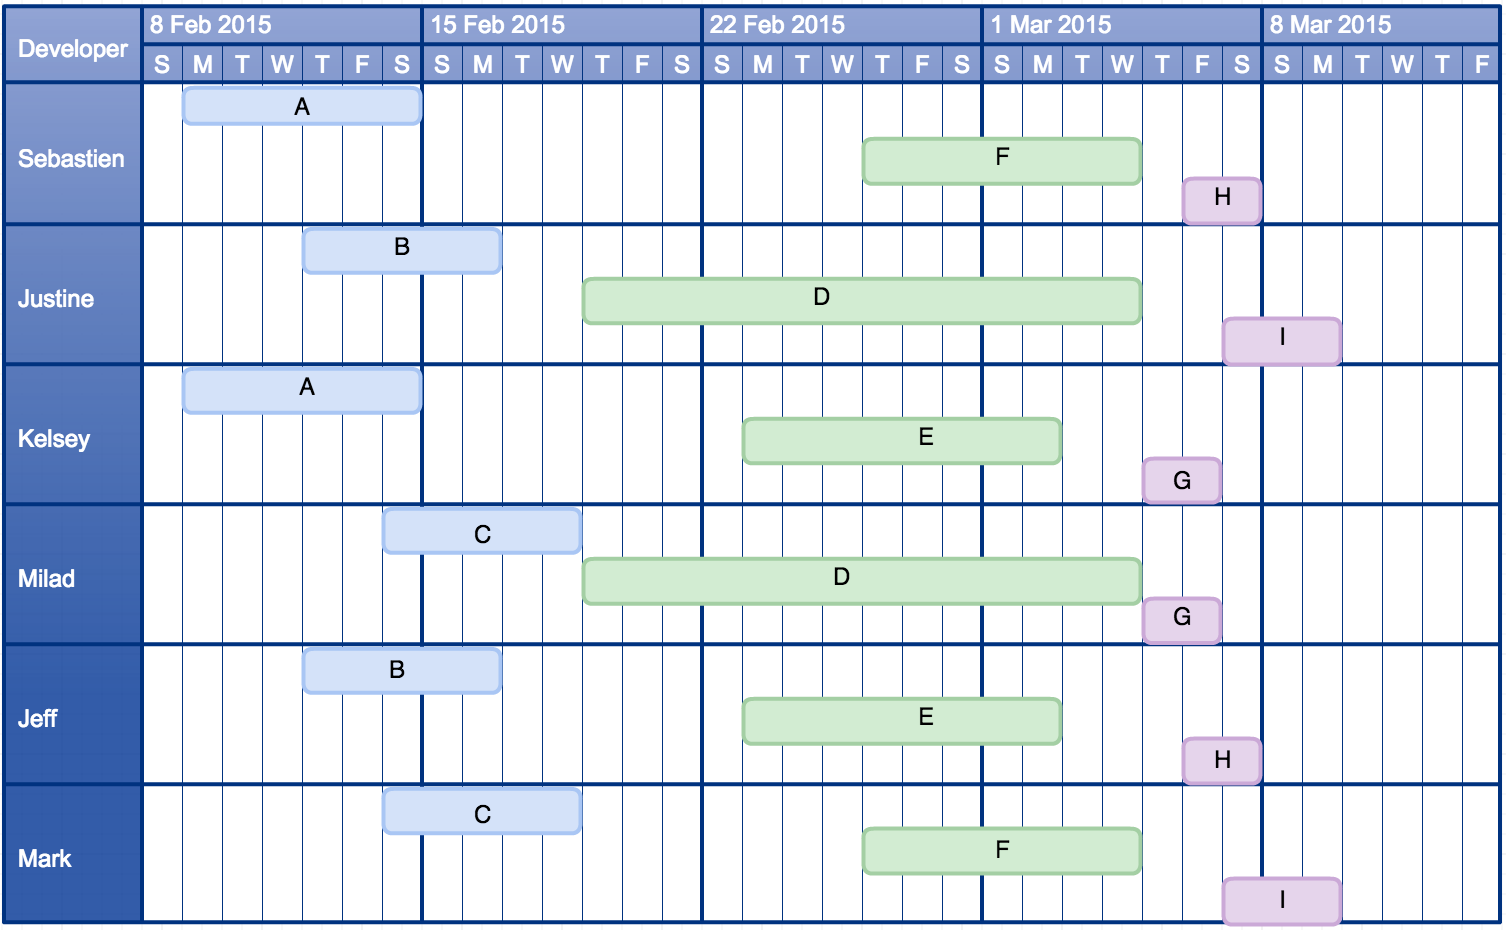
\includegraphics{StaffAllocation.png}
\caption{Staff Allocation}
\end{figure}

To re-iterate the information from the above chart taken from the PMP,
and to conform the the following sub sections presentation of changes to
the assigned milestones, refer to the below list of milestones and
assignees: \emph{D: Justine, Milad }E: Kelsey, Jeff *F: Mark, Sebastien

\subsection{3.3 Current Milestone Assignments and
Deviations}\label{current-milestone-assignments-and-deviations}

\subsubsection{3.3.1 Milestone
Deviations}\label{milestone-deviations}

Changes made to milestone assignees: * D: Sebastien/Justine * E:
Sebastien/Kelsey * F: Sebastien

The above changes in assignees were a direct consequence of changes to a
team member's expected contribution to the implementation. Milad
Gueramian did not have access to the required development tools due to
the loss of visual output from his Hewlett Packard laptop computer which
was expected for use in development of software covered in milestone D.
Consequently, it became necessary to send the machine in for repairs and
this team member's role was repurposed, which is explained later in this
section.

Added milestones not specifically accounted for in the PMP: * (New)
Backend: Mark * (New) Documentation: Milad, Jeff

As mentioned before, the PMP states that the development team process
relies on a principle of matching member tasks based on his/her level of
prior experience. Through the evolution of our processes, the
development team, in an effort to be efficient, relies ever more on this
principle. While the time allocation and estimation of milestones D-F
were correct at the conception of the PMP, articulation of specific
details were not. Therefore, new milestones have since been added to
clearly separate and assign tasks to the appropriate team member based
on prior experience. Furthermore, the task for the creation of this
document was not specifically taken into account in the PMP.
Consequently, Jeff Kang and Milad Gueramian-due to the latter's
inability to contribute to milestone D-were reassigned to the new
Documentation milestone.

\subsubsection{3.3.2 Deviations in Project Monitoring
Plan}\label{deviations-in-project-monitoring-plan}

\textbf{Issue Tracking on Github} In section 5.4 of the PMP, it is
stated that the Github.com issue tracking system will be used to monitor
milestones. Indeed, this is a fitting management and documentation tool
since the future maintainers of the code base will want to have access
to the development history of the software. The milestones and assignees
were not added in this system until very recently and all at once, which
is not ideal because there is no smooth timeline documenting events as
they occurred. However, section 5.4 also indicates that Google Docs will
be used as a means of tracking issues. This is still true and has helped
the development team to accurately keep track of issues and milestones
and to retroactively add them in the Github issue tracker and progress
reporting system. Furthermore, other communication methods described in
earlier documents such as a group text messaging thread and a Google
email messaging thread have been useful in keeping track of progress.
Therefore, the effects of this deviation were not detrimental in making
the planned progress.

\subsubsection{3.3.3 Deviations Caused By Change in
Timeline}\label{deviations-caused-by-change-in-timeline}

The client pushed up the due date for the product implementation
deliverable from Wednesday March 4, 2015 to Monday March 2, 2015. This
put considerable constraints on the development team in completing the
milestones set for the original due date at the time of the new, March 2
due date. Consequently, the development team decided to deviate plans
for adding some added advantages and assurances to the client and
software. Sphinx as a documentation management tool, outlined in section
5.1 of the PMP, will not be used. The impact of this deviation is that
the documentation provided by Sphinx form the source code comments will
not be created and therefor not available on the code base in Github.

Testing efforts were also affected by the constrained timeline. The
tests were not as inclusive as was previously planned. Because of the
earlier due date, quality assurance is hampered because we did not have
the necessary time to achieve full coverage of test cases. As stated in
section 5.3 of the PMP on software quality assurance, we wanted to adopt
the Test Driven Development Methodology because, ``this aims to provide
an additional measure for the advancement of the project as well as an
assurance on its quality,'' the shorter deadline did not allow for this
to happen. As a result, JSCoverage was not used because our tests were
not as strong as we expected.

\subsubsection{3.3.4 Quality Assurance}\label{quality-assurance}

Travis CI was used in conjunction with Github allowing continuous
integration along the process of the limited testing which we did
perform. These limited tests were very simple however. PHP\_Unit was
also used as a code coverage tool as reported in section 5.3 (Quality
Assurance Plan section) of the PMP. Refer to the Appendix 6.1.2 for
updates on milestone from the Github issue tracker that was used, as
stated in the management plan, as a means to track progress.

Our custom progress metric and measurement system as described in the
PMP was deployed with success. Each group member of the development team
rated the progress of other members on assigned milestones and the
totals were averaged as described in the PMP. These are internal
controls that were recorded on the whiteboard of the room used for
weekly (sometimes bi-weekly) group meetings. Progress was effectively
tracked so the development team was aware of overall performance.

Additionally, progress of the individuals who coded the program was
measured by assigning primary and secondary coders. The primary was the
individual assigned to implement a function, and the secondary was the
coder who double checked their work. This was a measure of how
efficiency of implementation was accounted for to make sure the C-Lyrics
system would work.

\section{4 Risk Monitoring Plan
Adherence}\label{risk-monitoring-plan-adherence}

The risks identified in section 6.1 of the PMP helped prepare the
development team for the event that a team member becomes incapable of
working. A team member did not have access to his laptop and development
software and environments due to a broken screen. This caused the team
to change and re-assign some milestones as noted in the deviations
sections above. The changes were tolerable because this risk had been
accounted for in Contingency Plan \#4 of the PMP. Contingency plan \#4
also helped in creating some new milestones and re-assigning others
because the earlier estimations in the PMP were inaccurate in that the
work was not spread out efficiently and the documentation process for
the project was not taken into account as separate milestones. These
``new and re-assigned milestones'' are described in section 3 of this
document outlining deviations from milestones and listing current
milestones.

Furthermore, we accounted for the risk of not having a complete
implementation by the due date. We resorted to Contingency Plan \#6 in
our first submission of the product since some parts were not
implemented. Refer to Appendix 6.1.2 to see the functionality that is
missing and how this issue was tracked and maintained by the development
team.

\section{5 Startup Instructions}\label{startup-instructions}

\begin{itemize}
\itemsep1pt\parskip0pt\parsep0pt
\item
  Open the virtual machine image provided in the submission.
\item
  Execute the command ``sudo /opt/lampp/lampp start'' (without the
  quotation marks) and open your favorite browser to the following
  address: http://localhost/dist
\item
  Hopefully the website should appear. Please note that the application,
  especially the communication to the server, might feel a bit sluggish.
  This is probably due to latency problems between the machine and the
  API, however such problems should disappear as the application is
  deployed to a production server.
\end{itemize}

\section{6. Appendices}\label{appendices}

\subsection{6.1 Issue Tracking And Progress
Reporting}\label{issue-tracking-and-progress-reporting}

\subsubsection{6.1.1 Gmail Communications}\label{gmail-communications}

From: Sebastien Arnold, February 28, 2015

So, I just pushed some code on the organization repo.
(https://github.com/C-Lyrics/frontend) It is not fully working yet, and
there are still a few things to implement, but we are in good shape.
From what I understood, Mark has been making some progress as well on
the PHP, but we have troubles getting the actual lyrics for a given
song, as well as performance issues.

Performance should not be that much of a problem, as we can always speed
things up. Regarding the songs issue, I found two unofficial APIs for
RapGenius:
http://blog.edforson.me/introducing-genius-api-rapgenius-api-as-a-service/
and more complete, but more difficult to understand:
http://api.genius.com/search?q=the+recipe

It would be very good if we could have the backend online as well, on
the repo of the organization. So that we can have a look at how we want
to integrate both parts of the application. You should all be invited to
join, if you were not shoot me an email.

Also, someone should begin to take of the document we have to submit for
the implementation. Milad, I suggest you do it, that will be easier for
you than to code stuff, as you don't have your usual tools for coding.

From Mark Krant, February 28, 2015 Just committed the back end. It
works, but to an extent. Since I could not find a free lyrics API, I
used a webscraper framework to go to a page for each song by an artist
and get the lyrics from there. Only problem is that it takes way too
long, and Sebastien said it can be done using asynchronous calls, but I
still need to look into that more because I have no idea how to do that.
A band with like 15-20 songs might take 10-15 seconds to load, but 150+
songs will cause it to time-out (it times out after 120 seconds). If
anyone has suggestions / knows how to do it feel free to edit the code.
It is under /backend/templates/getSongs.php

Also I did not do error checking for the back end yet. So if you try to
make a word cloud with an artist name ``sdfgh'' then it will blow up.
it's a quick fix so ill do it soon

\subsubsection{6.1.2 Milestone
Tracking}\label{milestone-tracking}

Below are the two issues relating to unimplemented functions from the
first product submission.


\begin{figure}[htbp]
\centering
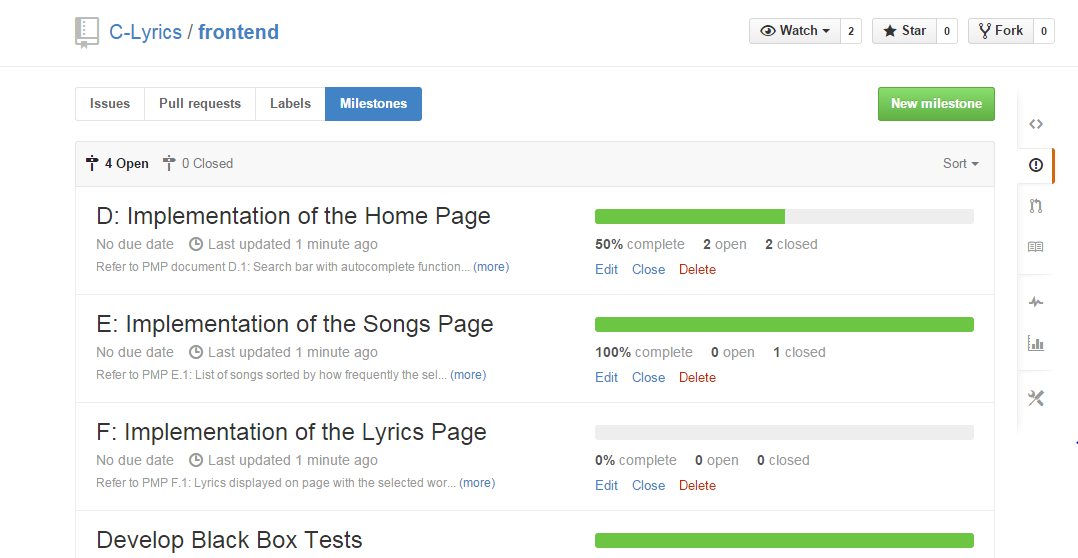
\includegraphics{milestones1.png}
\caption{Milestones, part 1}
\end{figure}


\begin{figure}[htbp]
\centering
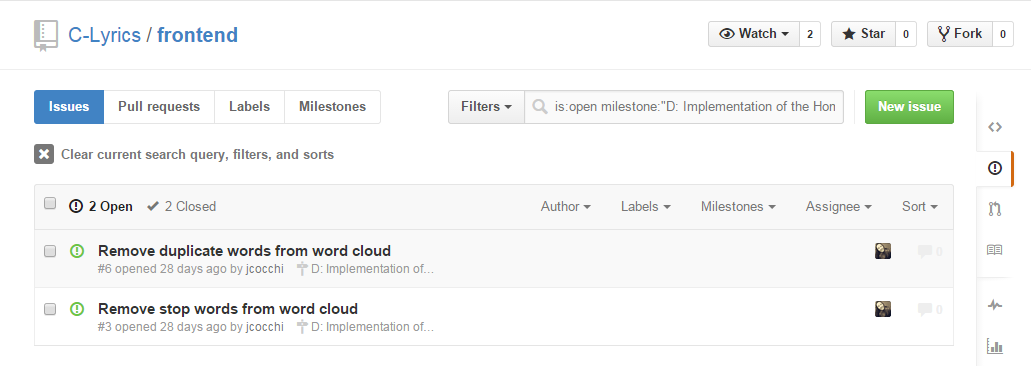
\includegraphics{milestones2.png}
\caption{Milestones, part 2}
\end{figure}

\end{document}
